\documentclass[a4paper, english, 12pt]{article}
\usepackage[utf8]{inputenc}
\usepackage[norsk]{babel}
\usepackage{mathtools}
\usepackage{hyperref}
\usepackage{listings}
\usepackage{graphicx}
\usepackage{float}

\begin{document}
\begin{titlepage}
\begin{center} 

\vspace*{3cm}
\textsc{\Huge PU1}\\[0.7cm]
\textsc{\medium TTM4100 - Communication Services and Networks}\\[0.3cm]
\textsc{\medium TDT4140 - Software Enigneering}\\[0.3cm]
\textsc{\medium TDT4145 - Data Modeling, Databases and Database Management Systems}\\[0.3cm]
\textsc{\medium TDT4180 - Human-Computer Interaction}\\[0.3cm]

\textbf{\Large Gruppe 7:} \\[0.2cm]
\text{\Large Espen Albert, Finn Inderhaug, Kristoffer Andreas Dalby} \\
\text{\Large Christoffer B. Nysæter, Andreas Wien, Jonas André Dalseth}\\[1cm] 

\today

\end{center}
\end{titlepage}

\section{Resources}
We have 6 persons available for completing the application. Every person has their own personal computer with  development tools for the \href{http://www.oracle.com/technetwork/java/javase/downloads/java-se-jre-7-download-432155.html}{java runtime environment}, the \href{http://www.postgresql.org/}{postgreSQL} database, 
and the \href{http://json.org/}{JSON} object interface.
The budget for our project is limited to the work hours specified in time estimate.

\section{Time and budget estimate}
Based on the resources we have at our disposal we have made the following time and budget estimates.
Since this project is a school exercise labour is free. Nonetheless we have put together a budget consisting of our work hours and a fictive salary of $849,90 NOK$. Making the salary budget a total of $\approx 734300 NOK$. In addition to creating a calendar, we have also been given a separate project in TTM4100 which we have included here, and will take some of the total work time.
We have estimated a total monetary spending budget of 0 NOK, because we are using free software and the developers personal computers. It is highly unlikely that we will pay for any new software or hardware during this project. 

We have estimated 18 workdays of 8 hours, with 6 developers. This gives us $864$ work hours.

\section{Deadlines}
The absolute deadlines are required from our customer(the exercise) are shown in table \ref{deadline}.

\begin{table}[h!]
    \begin{center}
    \caption{Deadlines} 
    \label{deadline}
    \vspace{0,5cm}
    \begin{tabular}{| l | l |}  
        \hline
        Task & Due by date \\
        \hline 
    PU1  Prosjektplan & 2.mars \\
    PU2  Systemtestplan & 2.mars\\
    KTN  Prosjektplan & 3.mars\\
    DB   ER modell& 6.mars\\
    MMI  D2.1 og 2.2 & 7.mars\\
    PU3  Overordnet Design & 9.mars\\
    DB2  Logisk databaseskjema & 14.mars\\
    MMI  del 3 & 14.mars\\
    PU4  Implementasjon og testing & 21.mars\\
    PU5  Dokumentasjon & 21.mars\\
    KTN  working implementation & 24.mars\\
        \hline
    \end{tabular}
    \end{center}
\end{table}



\section{Responsibilities}
We will divide the responsibility for the completion of the exercise in 4 parts; the database, network communication, client model and client view.  There is also a person responsible for human resources, and a union representative chosen democratically by the group. The human resource responsible has taken on him to create a friendly work environment and to plan fun excursions.

\subsection{Database}
The database will hold every piece of information that the program needs to save over a longer time period. The work is divided as shown in table \ref{database}


\begin{table}[h!]
    \begin{center}
    \caption{Database section and amount of time} 
    \label{database}
    \vspace{0,5cm}
    \begin{tabular}{ll} \\ 
        \hline
        $Task$ & $Estimated hours$\\
        \hline 
    Create ER-diagram for the application & 10 hours\\
    Logic databasechema & 10 hours\\    
    Setup the database server & 8 hours\\
    Create the needed structure in SQL & 16 hours\\
    Implement JDBC & 8 hours\\
    Implement needed methods & 16 hours\\
    \hline 
    Total & 68 hours \\
    \hline
    \end{tabular}
    \end{center}
\end{table}

\subsection{Network communication}
Network communication consists of the part of the server communicating with both clients and the database. It is vital that the server can lock resources, and still queue requests from clients. In table \ref{Network} we have a look at how many work hours that will be allocated to this part of the system.

\subsection{Network communication}
\begin{table}[h!]
    \begin{center}
    \caption{Computer networking work breakdown schedule}
    \label{Network}
    \vspace{0,5cm}
    \begin{tabular}{ll} \\
        \hline
        $Task$  & $Estimated hours$ \\
        \hline
Creating a class diagram & 4 \\
Sequence diagram for login, send message from client and logout. & 6 \\
A short textual description of the design & 2 \\
Play with JSON & 6 \\
Server and client login & 6\\
Server and client logout & 6\\
Extra functionality & 0-24 \\
System integration & 10 \\
Test many clients & 4 \\
Overall computer networking separate project & 44 \\
\hline
Planning server to client & 6 \\
Planning client to server & 6 \\
Server to clients, Master & 10 \\
Server and clients, Threads sending JSON objects to logged in clients & 16\\
Clients to server, Master & 10\\
Clients to server, Check for inconsistency & 10\\
Clients to server, multiple Threads & 10\\
Overall computer networking common project total& 58 \\
\hline
Overall computer networking total & 102 \\
        \hline
    \end{tabular}
    \end{center}
\end{table}


\subsection{Client model}
The client model can be separated in to several smaller problems that are easier time estimated as parts. The sum of these makes the total time estimate of the clients model as seen in table \ref{clientmodel}. The model will be written in java, and handle json objects from the server. It will also provide a fully fledged API for the GUI\footnote{graphical unit inteface}. 

 \begin{table}[h!]
    \begin{center}
    \caption{Client model time estimate} 
    \label{clientmodel}
    \vspace{0,5cm}
    \begin{tabular}{ll} \\ 
        \hline
        Task & Estimated hours\\
        \hline 
    Creating login functionality & 7 \\
    Parsing json objects to model & 8 \\
    Define model and API structure  & 12\\
    Create json objects based on the model & 8 \\
    Creating vital functions and objects & 16 \\
    Create unit tests & 6 \\
    Optimize the notify function & 15 \\    
        \hline
    Sum & 72\\
    \hline
    \end{tabular}
    \end{center}
\end{table}



\subsection{Client view}
The client view is the way the user interacts with the system. It features an easy to use interface communicating with the clients model. The workload is shown in table \ref{UI}.

\begin{table}[h!]
    \begin{center}
    \caption{Time to design the user interface} 
    \label{UI}
    \vspace{0,5cm}
    \begin{tabular}{ll} \\ 
        \hline
        $Task$ & $Estimated hours$\\
        \hline 
    Discuss how we want the user interface & 12 hours\\
    Designing the user interface using paper models & 12 hours\\    
    Show papermodel to studass and another group & 6 hours\\
    Fix papermodel after feedback & 3 hours\\
    Conceptual model & 6 hours\\
    Screen design & 12 hours\\
    Construction design & 12 hours\\
    Make login screen & 4 hours\\
    Make appointment view & 16 hours\\
    Make week view & 16 hours\\
    Other functionality & 16 hours\\
        \hline
    \end{tabular}
    \end{center}
\end{table}
\section{Work load distribution as gantt diagram}
We are planning on rotating the tasks between people. The persons responsible are listed in table \ref{responsible}.
\begin{table}[h]
    \begin{center}
    \caption{Responsibilities} 
    \label{responsible}
    \vspace{0,5cm}
    \begin{tabular}{ll} \\ 
        \hline
        $Person$ & $Responsibilities$\\
        \hline 
        Espen Albert & Network communication\\
        Finn Inderhaug Holme & Client model\\
        Kristoffer Kradalby & Database \\
        Jonas André Dalseth & Client ciew, human resources \\
        Andreas Wien & Union represntative\\
        \hline
    \end{tabular}
    \end{center}
\end{table}
Espen is responsible for the KTN separate project. He will be rotating between the KTN project and the other projects. He will take turns working with different parts of the project for example

\begin{itemize}
\item monday: KTN with Jonas.
\item tuesday: GUI with Jonas. 
\item wednesday: KTN with Kristoffer. 
\item thursday: Database with kristoffer. 
\end{itemize}
The documentation will be an ongoing project since day one. We will log hours and do documentation all the way. The work load is shown in figure \ref{gantt}

\begin{figure}[h!] 
    \begin{center} 
    	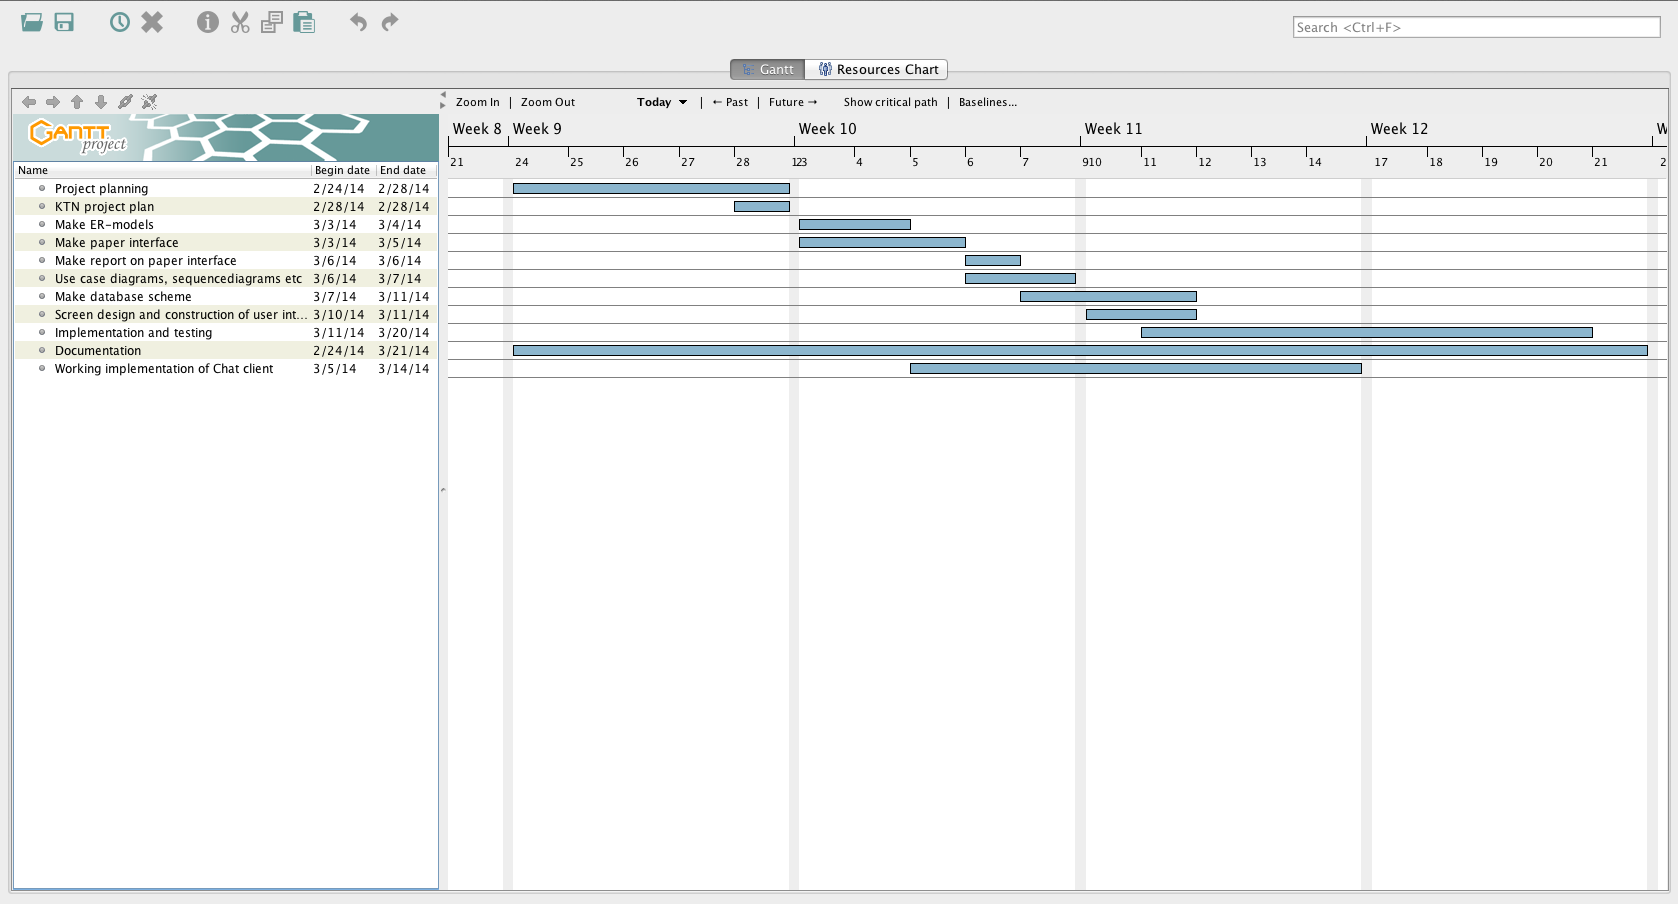
\includegraphics[width=15cm]{GanttDiagram.png}
		\caption{Gantt diagram}
	\label{gantt}
	\end{center}
\end{figure}

\section{Risk analysis}
Our simple risk analysis is shown in figure \ref{risk}. The overall workload distribution is way below the $860$ hours. We have accounted for pretty much everything not going as planned. 
\begin{figure}[h!] % 
    \begin{center} %
    	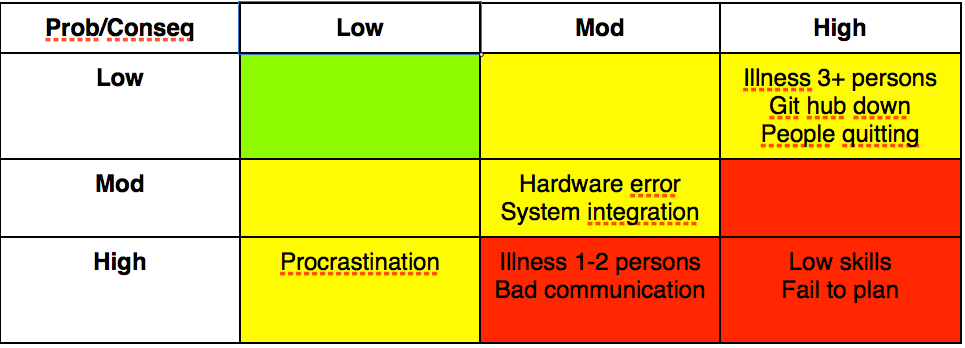
\includegraphics[width=8cm]{Risikoanalyse.png}
		\caption{Risk analysis}
	\label{risk}
	\end{center}
\end{figure}

                Procrastination , Focus on the task ahead, take brakes when needed , Extra work hours \\
        Hardware error , Only use stable packages, backup regularly , Loss of work \\
        System integration , Good communication between programmers , Extra work hours to resolve conflicts \\
        Illness , Vitamin c, don't overwork, enough sleep , take a day off\\
        Bad communication , have meetings, do social events together , extra hours due to miscommunication \\
        Loss of programmers due to serious illness , N/A , Talk to undass, lower goals \\
        Git hub down , keep backups , switch to PVV's gitlab \\
        People quitting , be nice to them , Talk to undass, lower goals\\
        Low skills , Read curriculum in courses , Help each other, or ask studass \\
        Fail to plan , We have several hours in reserve that can be used , Ask undass, lower goals\\
        



\end{document}
